\section{Methodology} \label{isect2}
\subsection{Existing approaches and related literature}
\subsubsection{Theoritical Review}
The main economic theory to study sustainable livelihoods was developed by Robert Chambers and Gordon Conway in mid 1980s. \cite{chambers1992sustainable} contends that a sustainable livelihood is one that can withstand stress and shock, maintain or improve its assets and capabilities, and create opportunities for future generations to live sustainably. It also generates benefits for other livelihoods both locally and globally as well as over the long term. The author created the Sustainable Livelihood Approach (SLA) for the purpose of evaluating various vulnerability contexts to improve the effectiveness of development cooperation.\par

Based on the Sustainable Livelihood Approach (SLA), the Sustainable Livelihood Framework (SLF) was proposed with a particular emphasis on the institutional processes which mediate the ability to carry out combination of livelihood strategies with the given livelihood resources in a particular context to achieve an outcome. Some of the well-known livelihood frameworks are those proposed by Department of International Department \cite{dfid1999sustainable}, \cite{ellis1999rural} and \cite{scoones2013livelihoods}.\par

\cite{dfid1999sustainable} defines livelihoods broadly and systematically, considering the various assets that individuals or communities can draw upon for sustainable living. It emphasizes the inter-linkage of various capitals (Human, Social, Financial, Physical, and Natural Capital) the households possess with the livelihood outcomes. The framework provides a holistic viewpoint by taking into consideration the dynamic exchange of the capitals and how they influence the result of livelihood.\par

\cite{ellis1999rural}  builds on the DFID model by introducing the idea of vulnerability and emphasizes the importance of understanding the factors that makes certain people or groups more vulnerable to shocks and stresses. The author highlights the significance of understanding the elements that make people or communities more vulnerable to shocks and pressures and presents the idea of vulnerability as a major predictor of livelihood strategies and results.\par

\cite{scoones2013livelihoods} contributed to SLF issue by emphasizing the importance of social relations and political economy in determining the livelihoods. The author's work highlights the need for critical analysis of social relations and political context and how they impact the household's ability to secure more sustainable livelihoods. The framework stress the need for a comprehensive understanding of livelihoods, taking into consideration not only the assets and vulnerability but also the the social, economic and political dimension.\par

In a nutshell, DFID framework provides a comprehensive overview of various capitals that impact livelihoods. It acknowledges the concept of vulnerability but doesn't make it a central focus. Also, it does not explicitly delve into social and political dimension of livelihoods. Ellis on the other side of the spectrum, introduces the concept of vulnerability and places a strong emphasis on understanding the elements that increase the likelihood of failure. The framework includes some consideration of political and institutional factors but is centered more on vulnerability. Scoone highlights the critical role of political economy and power structures in shaping the livelihoods. Each framework brings unique perspectives to the understanding of sustainable livelihoods, with varying levels of focus on capitals, vulnerability, political economy, and power dynamics.\par

\subsubsection{Household Vulnerability}
Vulnerability is a concept that is applied in various disciplines, including engineering, ecology, economics, psychology and sociology \citep{fang2016rural}. Vulnerability refers to a state in which a person feels insecure when something harmful occurs \citep{chambers2006vulnerability}. "Vulnerable" refers to something that is likely to be harmed or wounded in everyday language. The term "Vulnerable", which means "wound", is dervied from the Latin word "vulnerare," \citep{calvo2005measuring}. On a similar note, \cite{chambers1989editorial}  states that vulnerability “refers to exposure to contingencies and stress, which is defenselessness, meaning a lack of means to cope without damaging loss”.\par

The concept of household vulnerability is both controversial and multifaceted \citep{zhang2020capital}. So, household vulnerability analysis requires identification of not only the threat, but also the ‘resilience’, or responsiveness, in exploiting opportunities, and in resisting, or recovering from, the negative consequences of a changing environment \citep{moser1998asset}. In this perspective, \cite{bernier2014resilience} defines the resilience as the ability of a person, household, community, or system to adapt over time to shocks and proactively lower the risk of future shocks is what we refer to as resilience; these efforts promote growth and development as opposed to stability.\par

Many scholars conceptualise resilience as capacities that are driven by a set of capitals to produce outcomes such as influencing preparedness, mitigating impacts, and enhancing recovery against some risks. \cite{gaisie2021complexity} reveals complex relationship between household capitals and disaster outcomes in Ghana. The study finds that household capitals indicating higher economic status were linked to worse impacts from flooding but were essential for facilitating household recovery over time. \cite{zhang2020capital} in the similar study conducted in China suggests that all forms of capital (financial, human, natural, physical, and social 
capital) of a household were important determinants of household vulnerability. The term "resilience" and "vulnerability" has been used in the literature as antonyms of one another. The basic concept is that the more resilient a system, the less vulnerable it is.\par 

\cite{fang2016rural}, by constructing a composite vulnerability index, assessed the household vulnerability of the households in Shigatze Prefecture in Tibet
Autonomous Region (TAR) in China. The index has been constructed by taking into account the factors such as food variability, literacy rate of labor force, cash income and expenditure, precipitation vulnerability and drought area. The study finds that the factors under consideration reflects the close relationship between the basic requirement of th rural households in te harsh plataeu environment, less developed regions and vulnerability.\par    

\cite{antwi2013characterising} assessed the vulnerability to drought across six communities in Ghana. The study reveals varying vulnerability degrees influenced by socioeconomic factors. Authors find that less vulnerable households depict the resilience through alternative livelihoods and social connections. On a similar study, \cite{rahman2023households} quantifies cyclone vulnerability in rural Bangladesh, emphasizing  the multidimensional nature of vulnerability encompassing social, economic, physical, institutional, environmental, and attitudinal factors. The research, focusing on Kalmegha and Patharghata regions, reveals distinct vulnerability patterns, particularly in environmental and composite aspects. \cite{notenbaert2013derivation} constructed the household vulnerability index and explores the vulnerability and coping capacity related to current variability conditions with  focus on the adaptive capacity of the households. The study suggests that distance to paved road, income diversification and savings of the households significantly influences the household vulnerability.\par
\subsubsection{Review of National Studies}
Numerous studies have been conducted with respect to the assessment of vulnerability across Nepal. The following study uses the country-level data to investigate the vulnerability. \cite{aksha2019analysis} investigated the social vulnerability in Nepal by adapting Social Vulnerability Index (SoVI) methods to Nepalese context using the full data set of 2011 census provided by the Central Bureau of Statistics (CBS). The study employs the Principal Component Analysis (PCA) to generate the independent set of factors to calculate the SoVI score. The SoVI for Nepal was calculated for each spatial unit (3918 village development committee and 53 municipalities). The components used in the study are renters and occupation, poverty and poor infrastructure, favorable social conditions, migration and gender, ethnicity, medical services, education. The study finds that social vulnerability is particularly high in areas that have concentrations of Dalit and Minority populations.\par    

\cite{shahiestimating} estimate the vulnerability score for Nepal using a three-stage feasible generalized least square technique to assess vulnerability to poverty. Utilizing the third round of Nepal Living Standards Survey data, the study's findings reveal that Nepal's overall vulnerability is 33 percent, indicating the probability of households falling into poverty due to various shocks such as death, illness, unemployment, and other idiosyncratic factors. The vulnerability score is notably high for minority populations. The authors identify Karnali and Sudurpaschhim regions as having a higher proportion of highly vulnerable households.\par 

On a household level, \cite{bista2019grasping} examines the relationship between the magnitude of climate variability and household vulnerability in the catchment areas of the Sot Khola sub-water basin in the western mountainous region of Surkhet, Nepal. The author constructs a theoretical climate vulnerability index based on household-level data collected from 642 households, covering adaptive capacity, sensitivity, and exposure. The findings reveal that a majority, 52.7\%, of households are sensitive to climate-induced disasters such as landslides and floods due to their socio-economic status and food insufficiency. The study suggests that, overall, 67\% of households are vulnerable to varying degrees, ranging from moderate to extremely high vulnerability, while the remaining 33\% are least vulnerable.\par


Another household survey study by \cite{mainali2019mapping} employs a mixed-method approach, utilizing the Livelihood Vulnerability Index (LVI) at the community level. By integrating data from over 900 household surveys and national-level databases, the authors map the climate vulnerability of ten drought-prone villages in the central-east mid-hill region of Nepal. The findings reveal significant spatial variation in vulnerability, even within the lowest administrative units. Livelihood strategies, water availability, and topographic factors were among the key determinants of vulnerability, with strong interconnections among these components.\par 

A study by \cite{gerlitz2017multidimensional} based on Hindu Kush Himalayas (HKH) collects data from 2311 households from six districts (Khotang, Udaypur, Siraha, Dolakha, Sunsari, Kavrepalanchok) in Koshi sub-basin in Nepal and computes the Multi-dimensional Livelihood Index (MLVI). The MLVI was constructed using  AF method (Alkire \& Foster, 2011). Several variables as an indicator of Adaptive capacity, Sensitivity and Exposure has been employed to form a composite MLVI. The author finds, among the six districts, Khotang showed the highest multidimensional livelihood vulnerability with 96\% of the population were multidimensionally vulnerable to change and on average vulnerable in regard to 52\% of the 25 vulnerability indicators, resulting in an index value of 0.50.  Udayapur district showed the highest absolute contribution of lack of adaptive capacity to livelihood vulnerability 0.16.\par
 
\subsection{Household Vulnerability Index} \label{subsec:HVI}
A household confronted with a difficult situation is at risk of potential future declines in welfare. Vulnerability, which is the probability of encountering future loss of welfare, typically takes into account the severity of anticipated losses. The level of vulnerability is influenced by both the nature of the risk and the household's capacity to address risk using the capitals they possess. Households face numerous uncertain events. A household is said to be vulnerable, if it doesn't have adequate resources or capitals, particularly when exposed to risky situations where the household needs to use the resources at their disposal. Those resources are capital or assets of the households. Having these resources not only helps the houeholds deal with uncertain events but also improve their livelihoods and lifestyles.\par 

To identify the different levels of vulnerability amongst the households in rural households, we construct the Household Vulnerability Index. Taking into the capitals that households possess, we construct an aggregated index which helps to identify the vulnerable households within the community. The capitals we use to construct the index are: Human; Physical; Social; Financial; and livelihood strategies.\par 

To ensure the comparability of indicators that were used in the construction of the
household vulnerability index, all indicators were standardised following the
\citep{watkins2007human} procedure of standardising indicators for life expectancy index. This
ensures that all indicators were normalised to have a relative position between 0 and 1. \par
All variables with different scales are normalized with the following Min-Max standardization 
(Equations 3.5 and 3.6). Min-Max normalization helps to resize/rescale all variables analogously 
(i.e., into one scale). Here, all values are scaled between 0 and 1. Equation (3.5) applies to 
variables positively associated with vulnerability, while 
equation (3.6) applies to variables negatively associated with vulnerability. This method has been widely used in the literature related to vulnerability assessment. \cite{fang2016rural, antwi2013characterising, karunarathne2020developing, huynh2018multi, dumenu2020social} are some of the literature that have employed mini-max/maxi-min normalization technique to construct the vulnerability index.\par

When the variable has upward functional relationship with vulnerability, normalization was done using (1) and when the variable has downward functional relationship with vulnerability, normalization was done using equation (2):
\begin{align}
	\text{X}_{\text{ij}} &= \frac{X_{\text{i}} - X_{\text{Minj}}}{X_{\text{Maxj}} - X_{\text{Minj}}} \tag{1} \\[1cm] 	
	\text{X}_{\text{ij}} &= \frac{X_{\text{Maxj}} - X_{\text{i}}}{X_{\text{Maxj}} - X_{\text{Minj}}} \tag{2}
\end{align} 
where X is the observed value of the variable related to household i in district j, and Xmax and Xmin are 
maximum and minimum values of each variable, respectively. After normalizing all variables, 
we used equation (3.7) to calculate the final normalized index for each key component.
\begin{align}
	\text{HVI}_{\text{Cij}} &= \frac{1}{n}\sum_{i=1}^{n}\text{X}_{\text{ij}} \tag{3}
\end{align}
where $\text{HVI}_{\text{Cij}}$ is one of the five key components for HH. The main elements include human capital (C1), physical capital (C2), social capital (C3), livelihood (C4) and financial capital (C5). 	$\text{index}_{\text{Hvi}}$
depicts the variables of the key component indexed by C for i household in j district (while n represents the number of variables for each component). We used equation (3.8) to 
calculate the overall Hvi for the HH.
\begin{align}
	\text{HVI}_{\text{ij}} &= \sum_{i=1}^{n}\text{HVI}_{\text{Cij}} \tag{4}
\end{align}
where HVI is the Multi-facet Composite Household Vulnerability Index for HH x. 
C represents the numbers of key components,  indicates the weighting schemes used for the 
composite index, and n ensures the number of key components. Table 3 illustrates the weighting 
schemes used for the composite index calculated.\par 
                                   
\subsection{Household Vulnerability and Environmental Dependence}
After we construct the index and identify the most and least vulnerable, we attempt to understand the effects of the factors that weren't included in the index construction. These variables represent the liability to a household. Environmental income is a semi-capital/semi-liability characteristics variable. Environmental income is the revenue that a household generates from forest as well as non-forest sources. The sources are natural forest, managed forest, plantations, agroforests, silvipasture, other agriculture land, other areas. The products are firewood, charcoal, poles and other building material, fodder, fish, fruits, vegetables, medicinal plants etc. Because the income from the environment is a predominant source of income for livelihoods of rural households, it can be a source of capital for those households who do not have adequate resources. But, on the other hand, it can also be a liability when depending solely on these sources. Particularly, in the context of climate change and environmental degradation, it can be a source of liability of households. So, we investigate the influence of Environmental dependence on the household vulnerability.\par

To examine the effect of Environmental dependence on Household vulnerability, this study employs panel estimation techniques, including pooled-OLS, fixed effects (FE), and random effects (RE) models. While simple pooled-OLS doesn't account for the time-specific or hosuehold-specific effects, the fixed effects and random effects models are designed to address such endogenity issues. Pooled-OLS is essentially a statistical regression analysis method that visually represents the relationship between data points and determines the best-fit line for a dataset. However, the fixed effects model is theoretically more suitable for cases involving unobservable individual  or household effects that may be correlated with the variables included in the model. Conversely, if individual effects are strictly uncorrelated with explanatory variables, the random effects model is a preferable choice \citep{hsiao2022analysis}.   Effect of Environmental dependence on household vulnerability is modeled using
following regression,
\vspace{-\baselineskip}
\begin{center}
	\begin{align}
		\mathit{HVI}_{i,t} &= \beta_{0} + \delta \mathit{\mathbf{ED}_{i,t}} + \mathbf{X}_{i,t} \beta + \mathbf{Z}_i \lambda + \mathbf{T}_t \delta_t + \boldsymbol{\epsilon}\tag{5}
	\end{align}
\end{center}
where, \textit{HVIi,t} is Household Vulnerability of $i^{th}$ household in \textit{t} year, \textit{EDi,t} is Environmental dependence, \textit{T} is year control variable, \textit{Xi,t} is the variables controlled for, which includes Dependency ratio, log of debt, count of shock experienced and \textit{Zi,t} represents control for time invariant
fixed effect such as district and VDCs and $\beta_{0}, \delta, \beta, \lambda, \delta_t$ are the parameter of the model.\par 

\subsection{Diagnostic Tests}

For each techniques of the Panel data analysis, we'll run few diagnostic tests to check for the effects to be included in the model such as Individual and Time effects. Also, we run the efficiency test for choosing between the models.\par 

\subsubsection{Individual Effects Test} 
We run the Pooled Ordinary Least Squares (OLS) regression model without considering individual effects. After obtaining the results from Pooled OLS regression, we conduct F-test to determine if there are significant individual effects (fixed effects) present in the model. We'll refer to the F-statistic and associated P-value to determine the presence of significant individual effects.  A low p-value suggests the presence of significant individual effects.\par 

\subsubsection{Time Fixed Effects Test}
We also test for if there are time effects in the model. For this, we run the Pooled Ordinary Least Squares (OLS) regression model without considering individual effects. After obtaining the results from Pooled OLS regression, we conduct the Lagrange Multiplier Test - \cite{honda1988size}. It will allow us to determine if there are significant time effects (fixed effects) present in the model. We'll refer to the t-statistic and associated P-value to determine the presence of significant individual effects.  A low p-value suggests the presence of significant time effects.\par 

\subsubsection{Breusch-Pagan Lagrange Multiplier (BPLM) Test}
This test is commonly referred to as Pool-ability test conducted for confirming if the cross-sectional unit in the panel has the same intercept or a different intercept. \cite{breusch1980lagrange} assesses the pool-ability of the data after incorporating the time and individual fixed effects. We'll analyze the test-statistic and associated p-value. A low p-value suggests that the data is not poolable, indicating the inadequacy of Pooled OLS regression. We'll go for Random effects (RE) regression if the p-value is low.

\subsubsection{Hausman Specification Test}
If the BP-LM test suggests that the data is not pool-able and suggests to go for Random Effects (RE) model, we'll run the RE regression. We'll also run the Fixed effects (FE) model to compare the result. After running both Random Effects (RE) and Fixed Effects (FE) models, conduct the Hausman Specification test \cite{hausman1978specification} to determine the efficient model. The test is to check whether the coefficients estimated by the two models are significantly different. We'll analyze the test statistic, typically a chi-square value, and assesses the associated p-value.\par 

\subsection{Data sources}
This study employs the A unique environmental augmented household-level livelihood panel dateset \citep{walelign2022unique} from
Nepal, Full Panel 2006-2012, produced by Tribhuvan University’s Institute of Forestry and the University of Copenhagen’s Department of Food and Resource Economics . It is a geographically representative survey spanning three main physio-graphic regions of Nepal. Data was collected in the districts of Chitwan (lowland), Kaski (mid-hills), and Mustang (mountains). Total of 507, 446 and 428 randomly sampled households were surveyed in the year 2006, 2009 and 2012 respectively. For the questionnaire (see \cite{larsen2014role}). \par

\begin{figure}[htb] 
	\centering
	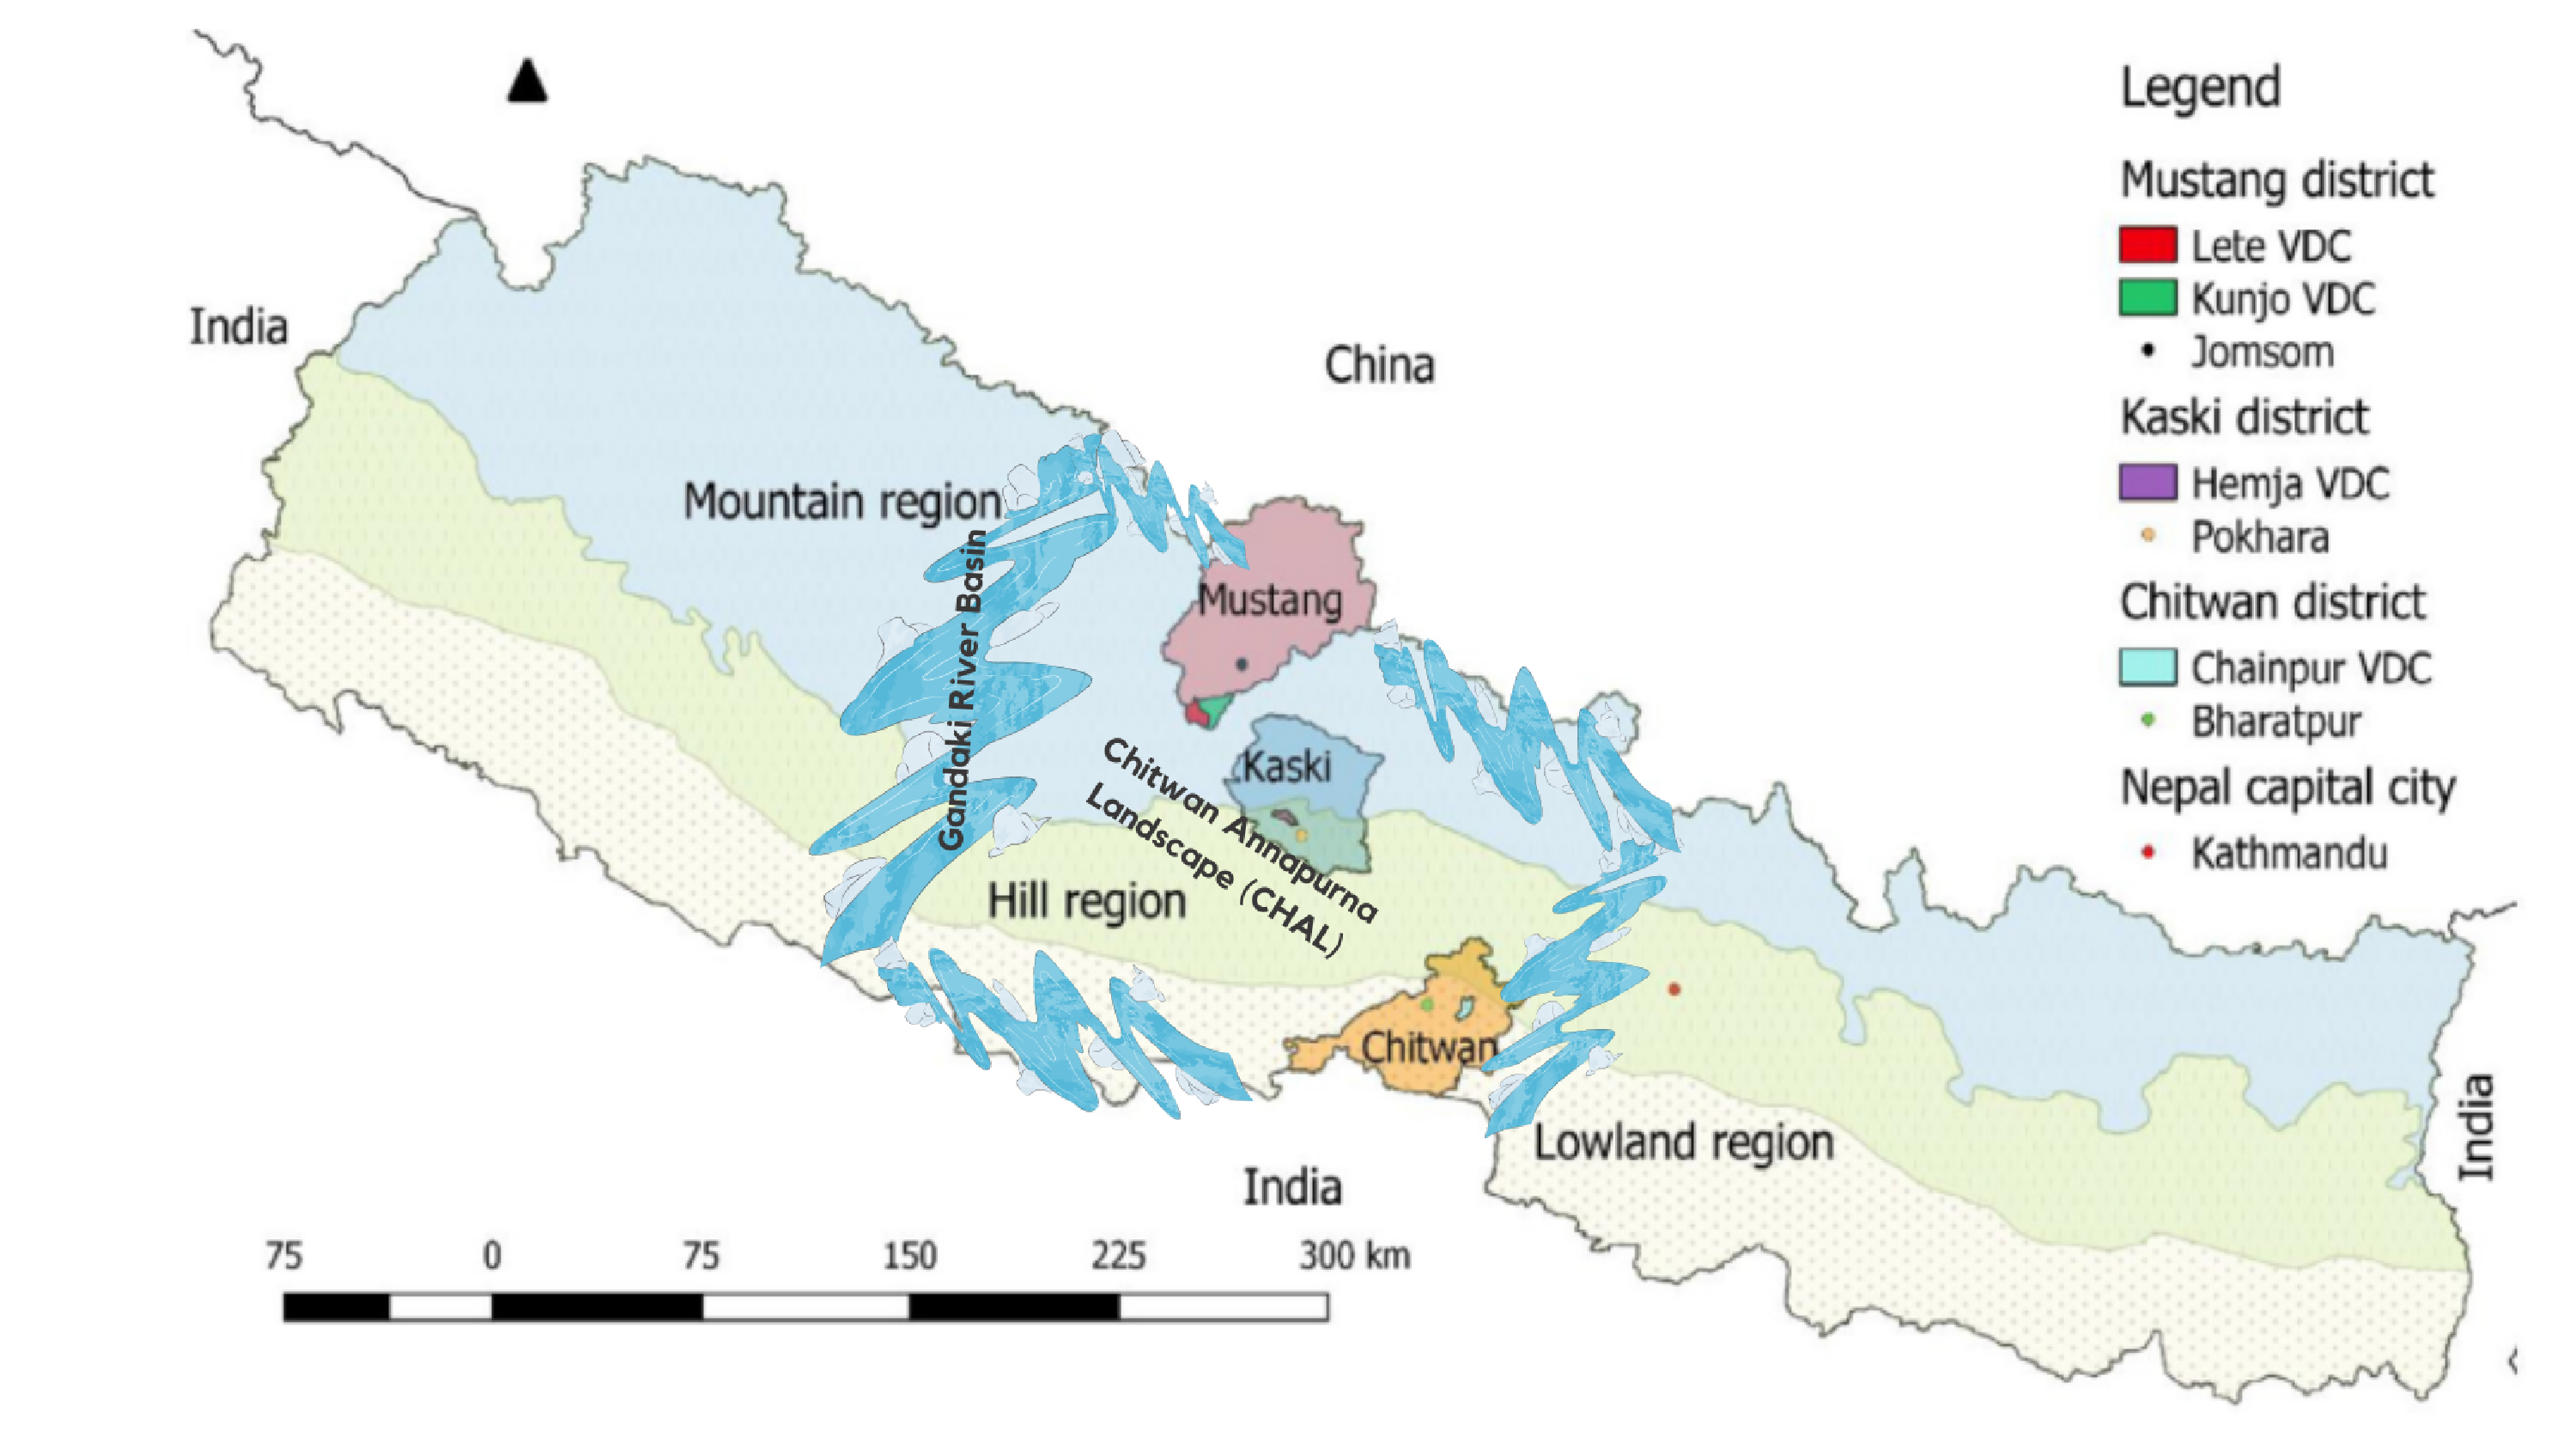
\includegraphics[scale=0.31]{./figure/Study site}
	\caption{Changes in real wage throughout the wage distribution (1998-2018)}
	\label{fig:wagechangeAll}
\end{figure} 

The three primary physio-graphic regions of Nepal—the lowlands, mid-hills, and mountains—are covered by the study sites. The selection factors included the following: (i) Nepal's changes in elevation and vegetation; (ii) the environmental reliance of households; (iii) the attitudes of communities toward long-term research; and (iv) village accessibility and researcher safety (because of the ongoing civil conflict in Nepal at the time of site selection in 2005).\par
The data was collected through the Community Based Forest Management in the Himalaya
(ComForM) phases I - III collaborative project conducted by the Institute of Forestry (IOF) at Tribhuvan University and the Department of Food and Resource Economics (IFRO) at the University
of Copenhagen, with support from the Department of Forest Research and Survey (DFRS) at the
Ministry of Forests and Soil Conservation, Nepal. The questionnaire design was developed together with the Poverty Environment Network (PEN).\par  

 
                            
